\documentclass{article}
\usepackage{tikz}
\usetikzlibrary{positioning}

\begin{document}

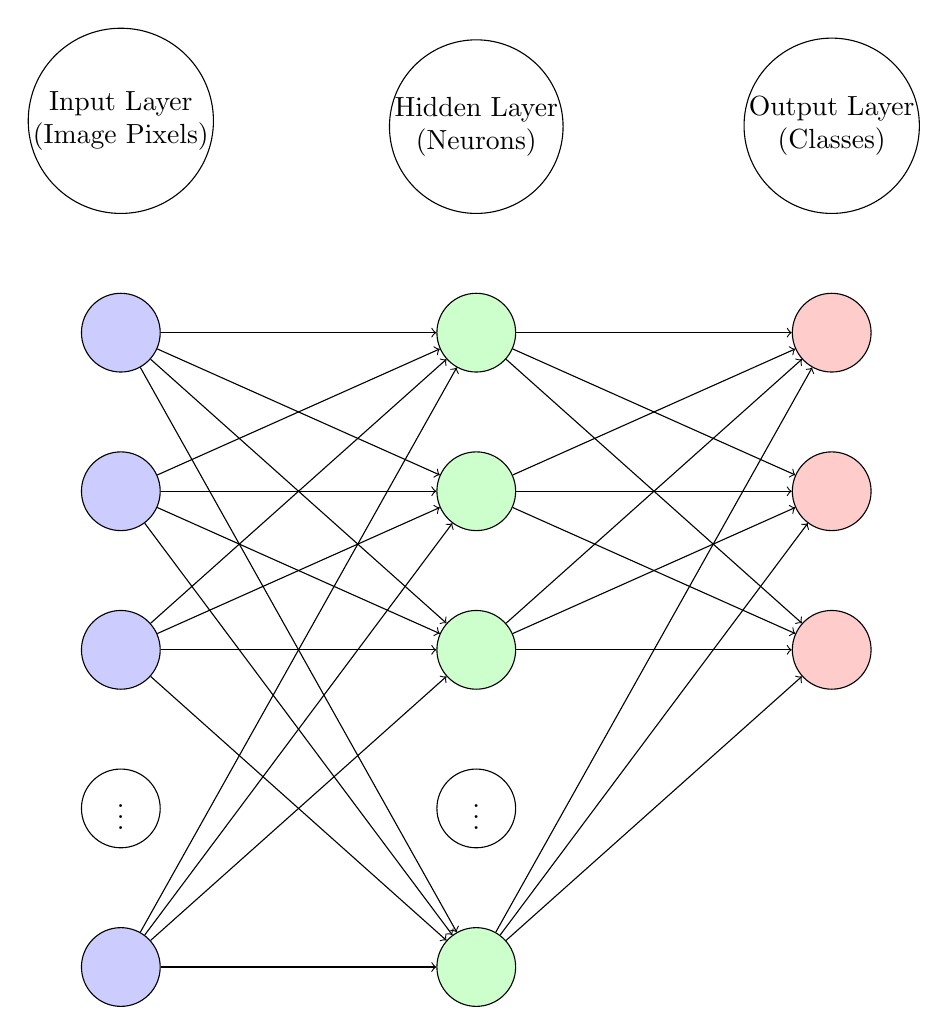
\begin{tikzpicture}[
    node distance=1cm and 1.5cm,
    every node/.style={draw, circle, minimum size=1cm, inner sep=0pt},
    input/.style={fill=blue!20},
    hidden/.style={fill=green!20},
    output/.style={fill=red!20},
    layer/.style={align=center}
]

% Input Layer
\node[input] (I1) {};
\node[input, below=of I1] (I2) {};
\node[input, below=of I2] (I3) {};
\node[below=of I3, node distance=1cm] (dots1) {\vdots};
\node[input, below=of dots1] (I4) {};

% Hidden Layer
\node[hidden, right=of I1, xshift=2cm] (H1) {};
\node[hidden, below=of H1] (H2) {};
\node[hidden, below=of H2] (H3) {};
\node[below=of H3, node distance=1cm] (dots2) {\vdots};
\node[hidden, below=of dots2] (H4) {};

% Output Layer
\node[output, right=of H1, xshift=2cm] (O1) {};
\node[output, below=of O1] (O2) {};
\node[output, below=of O2] (O3) {};

% Connections: Input to Hidden
\foreach \i in {1,2,3,4}
    \foreach \j in {1,2,3,4}
        \draw[->] (I\i) -- (H\j);

% Connections: Hidden to Output
\foreach \i in {1,2,3,4}
    \foreach \j in {1,2,3}
        \draw[->] (H\i) -- (O\j);

% Layer Labels
\node[layer, above=of I1, node distance=1.5cm] {Input Layer \\ (Image Pixels)};
\node[layer, above=of H1, node distance=1.5cm] {Hidden Layer \\ (Neurons)};
\node[layer, above=of O1, node distance=1.5cm] {Output Layer \\ (Classes)};

\end{tikzpicture}

\end{document}
